% ****** Start of file apssamp.tex ******
%
%   This file is part of the APS files in the REVTeX 4.1 distribution.
%   Version 4.1r of REVTeX, August 2010
%
%   Copyright (c) 2009, 2010 The American Physical Society.
%
%   See the REVTeX 4 README file for restrictions and more information.
%
% TeX'ing this file requires that you have AMS-LaTeX 2.0 installed
% as well as the rest of the prerequisites for REVTeX 4.1
%
% See the REVTeX 4 README file
% It also requires running BibTeX. The commands are as follows:
%
%  1)  latex apssamp.tex
%  2)  bibtex apssamp
%  3)  latex apssamp.tex
%  4)  latex apssamp.tex
%
\documentclass[%
%reprint for two column 
% preprint,
%superscriptaddress,
%groupedaddress,
%unsortedaddress,
%runinaddress,
%frontmatterverbose, 
%preprint,
%showpacs,preprintnumbers,
%nofootinbib,
%nobibnotes,
%bibnotes,
 amsmath,amssymb,
 aps,
%pra,
%prb,
%rmp,
%prstab,
%prstper,
%floatfix,
]{revtex4-1}

\usepackage{graphicx}% Include figure files
\usepackage{dcolumn}% Align table columns on decimal point
\usepackage{bm}% bold math

\renewcommand{\toprule}{\hline}
\newcommand{\midrule}{\hline}
\newcommand{\bottomrule}{\hline}

%\usepackage{hyperref}% add hypertext capabilities
%\usepackage[mathlines]{lineno}% Enable numbering of text and display math
%\linenumbers\relax % Commence numbering lines

%\usepackage[showframe,%Uncomment any one of the following lines to test 
%%scale=0.7, marginratio={1:1, 2:3}, ignoreall,% default settings
%%text={7in,10in},centering,
%%margin=1.5in,
%%total={6.5in,8.75in}, top=1.2in, left=0.9in, includefoot,
%%height=10in,a5paper,hmargin={3cm,0.8in},
%]{geometry}

\begin{document}

\preprint{ILD}


\title{The ILD detector at the ILC}% Force line breaks with \\
%\thanks{A footnote to the article title}%

\author{Editor Ties Behnke}
% \altaffiliation[Also at ]{Physics Department, XYZ University.}%Lines break automatically or can be forced with \\
%\author{Second Author}%
% \email{Second.Author@institution.edu}
\affiliation{DESY, Notkestrasse 65, 22607 Hamburg, Germany}
% Authors' institution and/or address\\
% This line break forced with \textbackslash\textbackslash
%}%

\collaboration{The ILD Concept Group}%\noaffiliation

%\author{ILD author list}
% \homepage{http://www.ilcild.org}
%\affiliation{
% Second institution and/or address\\
% This line break forced% with \\
%}%
%\affiliation{
% Third institution, the second for Charlie Author
%}%
%\author{Delta Author}
%\affiliation{%
% Authors' institution and/or address\\
% This line break forced with \textbackslash\textbackslash
%}%

%\collaboration{ILD Collaboration}%\noaffiliation

\date{\today}% It is always \today, today,
             %  but any date may be explicitly specified

\begin{abstract}
The international large detector, ILD, is a detector concept which has been developed for the electron-positron collider ILC. The detector has been optimised for precision physics in a range of energies between 90~GeV and 1~TeV. ILD features a high precision, large volume combined silicon and gaseous tracking system, together with a high granularity calorimeter all inside a solenoidal magnetic field. As a guiding principle in the design the concept of particle flow has been at the center of the deliberations. In this document the concept of the detector, the proposed implementation and the readiness of the different technologies needed for the implementation are discussed. The discussion takes place in the context of the ILC collider proposal, now under consideration in Japan, and includes site specific aspects needed to build and operate the detector at the proposed ILC site in Japan.

\begin{description}
\item[PACS numbers]
May be entered using the \verb+\pacs{#1}+ command.
\end{description}
\end{abstract}

\pacs{Valid PACS appear here}% PACS, the Physics and Astronomy
                             % Classification Scheme.
%\keywords{Suggested keywords}%Use showkeys class option if keyword
                              %display desired


\maketitle
%\tableofcontents

%\newpage

\section{\label{sec:level1}Introduction}
The International Large Detector, ILD, is a detector proposal for the international linear collider, ILC. In this paper, the considerations which have guided the ILD group in the design of the detector, are summarised. The main technological challenges for the realisation of the concept are described, and possible technological solutions are sketched. The ILD concept is supported by a broad and international community of scientists. 

After a brief history of the ILD concept, the main components of the detector are described, followed by a short summary of technological results. The overall performance of ILD is demonstrated with the help of a few fundamental performance numbers. 
\section{History of the ILD detector concept}
The ILD detector concept group was formed in 2007, as a merger from two earlier detector concepts for electron positron colliders, GLD~\cite{ild:bib:ref-gld} and LDC~\cite{ild:bib:ref-ldc}. GLD was a concept for the Asian Linear Collider, LDC for the TESLA linear collider proposal. Both detector concepts were similar in that they relied on a combination of silicon and gaseous tracking, combined with precision calorimetry, though in detail the solutions were rather different. Following the agreement by the international community to continue with only one linear collider concept, the ILC, the two concepts joined forces. During 2007 and 2008, an intense effort took place to re-define the new detector based on the work done in the two previous concept groups. 

At about the same time particle flow as a novel concept to reconstruct complex events at a collider had become more generally accepted - though a convincing experimental proof was still missing at this time. ILD decided nevertheless to adopt particle flow as the central guiding principle for its detector concept, and developed the ILD design around this assumption. For a review on particle flow, see e.g. \cite{ild:bib:PandoraPFA}.

The ILD concept underwent a number of international reviews, and was validated as one of two ILC detector concept groups. After the delivery of the ILD technical design report in 2014~\cite{Behnke:2013lya}, ILD re-organised its structure, to respond to the increasing likeliness that ILC as a project would be realised in Japan, and started a re-optimisation process to react to new technical developments, and to the quest for reducing the cost of the overall project. 

\section{The ILD detector design: requirements}
The science which will be done at the ILC has been summarised in a separate document~\cite{ILCESU1}. It is strongly dominated by the quest for ultimate precision in measurements of the properties of key particles like the Higgs boson, the weak gauge bosons, and, once the center of mass energy is beyond its production threshold, the top quark. A more detailed description of the ILD detector and its design philosophy is available in cite{Behnke:2013lya}.

The anticipated precision physics program~(see e.g. \cite{Fujii:2017vwa} for a recent summary) drives the requirements for the detector, essentially from two somewhat different assumptions. Many final states which will be analysed are fully hadronic final states, with many jets. Thus an excellent reconstruction of jets is essential, which basically translates into an excellent jet energy resolution. Many studies for example looking at the reconstruction of W and Z bosons suggest that a jet energy resolution around 3\% is needed to fully exploit the power of the collider. Such a resolution requires an improvement of performance, for example compared to the LHC detectors ATLAS or CMS of nearly a factor of two. The concept of particle flow is currently believed to be the only approach which can reach this level of precision. Particle flow requires the reconstruction of charged and neutral particles with excellent efficiency over a large solid angle, though at moderate individual resolution. Thus a tracker with outstanding efficiency is stressed, combined with a calorimeter capable of reconstructing neutral particles with high efficiency. For ILD the choice has been made to combine a large volume gaseous tracking system - which promises excellent efficiency combined with low mass - and a highly granular calorimeter both in the electromagnet and the hadronic section. To ease the linkage between the tracker and the calorimeter both tracker and calorimeter should be inside the coil. 

In contrast to this a number of highly relevant channels require the precise reconstruction of exclusive final states, for example, containing heavy flavour final states. This requires in addition very precise reconstruction of the decay vertices of long lived particles, and thus implies a high resolution vertexing system close to the interaction region. 
The excellent performance of the tracking system  depends critically on the amount of dead material in the ILD detector. The total material budget in ILD in front of the calorimeter should be below 10\% of a radiation length, for most of the solid angle.


In a similar way the show-case reaction of the recoil HZ analysis requires high precision tracking, to be able to reconstruct the two-muon decay of the Z boson, against which the Higgs recoils, with a precision not limited by detector resolution effects. This adds excellent momentum reconstruction precision to the list of requirements. 

The design of the ILD detector thus has been driven by the following requirements: 
\begin{itemize}
    \item {\bf Decay length resolution:} Excellent decay length resolution is important for the reconstruction of heavy flavour states, and to reject background. A resolution of $ 5 \mu m \oplus 10 \mu m / p(GeV/c)sin^{3/2}\theta$ has been defined as a goal. 
    \item {\bf Momentum resolution} A momentum resolution of $2 \times 10^{-5} \mathrm{GeV}^{-1}$ should be reached with the combined Silicon - TPC tracker, asymptotically at high momenta. Excellent tracking efficiency and maintaining very good momentum resolution down to lower momenta will be reached by an aggressive design to reduce the material budget in the detector. 
    \item {\bf Jet energy resolution} Using the paradigm of particle a jet energy resolution of $3\%$ for light flavour jets should be reached. The resolution is defined in reference uds jets, as the rms of the inner $90\%$ of the energy distribution. 
\end{itemize}


The main parameters of the ILD detector are summarised in Table~\ref{ild:tab:barrelpara}.



\begin{table}[th]
    \centering
    \begin{tabular}{|l|l|c|c|p{4cm}|}
    \toprule
        Technology & Detector & Start   & Stop & comment \\
        \midrule
Pixel detectors & Vertex & 16   & 60   & 3 double layers of Silicon pixel \\
& Forward tracking  & 220 & 230 & 2 Pixel disks \\
\midrule
Silicon strip   & SIT    & 153  & 300  & 2 double layers of SI pixel            \\
& Forward tracking  & 250 & 371 & 5 layers of Si strip\\
                & SET    & 1811 & 1900 & 2 layers of SI strip           \\
                & & & & \\
Gaseous tracking & TPC & 330 & 1808 & MPGD readout, 220 points along the track\\
\midrule
Silicon Tungsten Calo & ECAL option& 1843 & 2028 & 30 layers of $5\times5 mm^2$ pixel \\
& ECAL EC option & 2450 & 2635 & 30 layers of $5\times5 mm^2$ pixel \\
& Luminosity Calorimeter & & & \\
\midrule
Diamond Tungsten calorimeter & Beam Calorimeter & &&\\
\midrule
SiPM on Tile & ECAL option   & 1843 & 2028 & 30 layers, 5 mm strips, crossed\\
& ECAL EC option& 2450 & 2635 & 30 layers, 5 mm strips, crossed\\
             & HCAL option   & 2058 & 3410 & 48 layers, $3\time3 cm^2$ pixels\\
             & HCAL EC option& 2650 & 3937 & 48 layers, $3\time3 cm^2$ pixels\\
\midrule
RPC          & HCAL option   & 2058 & 3410 & 48 layers, $1 \times 1 cm^2$ pixel \\
& HCAL EC option & 2650 & 3937 & 48 layers, $1 \times 1 cm^2$ pixel\\
\midrule
SiPM on Scintillator bar & Muon & 4450 & 7755 & 14 layers \\
& Muon EC & 2560 & 7755 & 12 layers \\

        
%        Silicon SIT & 153& 300 & 2 layers of SI strip detectors& & & \\
%       TPC & 330 & 1808 & 220 points in TPC & & & \\
%        Silicon SET & 1811& & 2 layers of SI strip detector & & & \\
%        ECAL & 1843 & 2028 & Tungsten absorber, Si sensor, 30 layers, $5 \times 5 mm^2$ cells & 2450 & 2635 & \\
%             &      &      & Scintillator strips, crossed, 5 mm wide, 30 layers& & & \\
%        HCAL & 2058 & 3410 & RPC gas layers, $1 \times 1 cm^2 cells$, 48 layers& 2650 & 3937 & 48 layers \\
%             &      &      & SiPM on Sintillator layers, $3 \times 3 cm^2 cells$, 48 layers& & & \\
%        Muon & 4450 & 7755 & SiPM on Scintillator strips, 14 layers & 2560 & 7755 & 12 layers\\
\bottomrule
    \end{tabular}
    \caption{Key parameters of the ILD detector. All numbers are from~\cite{Behnke:2013lya}}
    \label{ild:tab:barrelpara}
\end{table}


In addition to the pure science driven performance numbers the detector will have to be able to operate in the ILC environment. Due to the extreme focusing of the two beams in the interaction region, so-called beamstrahlung is generated, which produces significant background in the detector. The magnetic field focuses the majority of the charged component of the beamstrahlung background into the forward region, but some fraction will still hit sensitive detector parts. This is particularly true for the innermost vertex detector layers, 


\section{Implementation of the ILD detector}
The ambitious requirements of the ILC detectors sparked a world-wide R\&D program to develop and demonstrate the different technologies needed. The R\&D was mostly coordinated and executed within so-called R\&D collaborations, which concentrated on particular technologies and sub-detector systems. These collaborations operated outside of the detector concept groups, and, in many cases, served several detector concept groups, sometimes even at more than one collider proposal. 

The ILD concept group from its beginning has collaborated very closely with these R\&D groups, and has organised the needed R\&D work through and with the R\&D collaborations. 

The ILD concept from its conception has been open to new technologies. 
In many cases no final decision on the technology has been taken at this time, but several options are maintained. In the current implementation ILD differentiates between options and alternatives. 
For a particular technology to be accepted as an option, it has to demonstrate a certain maturity, has to demonstrate key performance parameters through test beam experiments, and has to develop a concept which addresses the main questions of integrating the technology into a subdetector for ILD. Technologies which are less mature can still be considered alternatives, meaning technologies which offer a promise for improved performance and/ or lower cost, where some experimental evidence exists that this technology will eventually become a feasible option, but where the final validation is still missing. 

The ILD detector is a multi-purpose detector in which the different requirements are addressed by a combination of different sub-detector systems. The optimization for ultimate precision in the reconstruction of charged and neutral particles required that all major systems are contained within a strong solenoidal magnetic field. This field allows the measurement of the momentum of charged particles and removes low-energy background from the main part of the detector. Ultimate precision also requires that as little dead material as possible is introduced into the detector system, which pushes in particular the coil to the outside of the tracking and calorimeter system. A three-dimensional rendering of the detector is shown in figure~\ref{fig:ILD}.
\begin{figure}[tb]
 %\epsfysize=9.0cm
 \begin{center}
 \begin{tabular}{lr}
 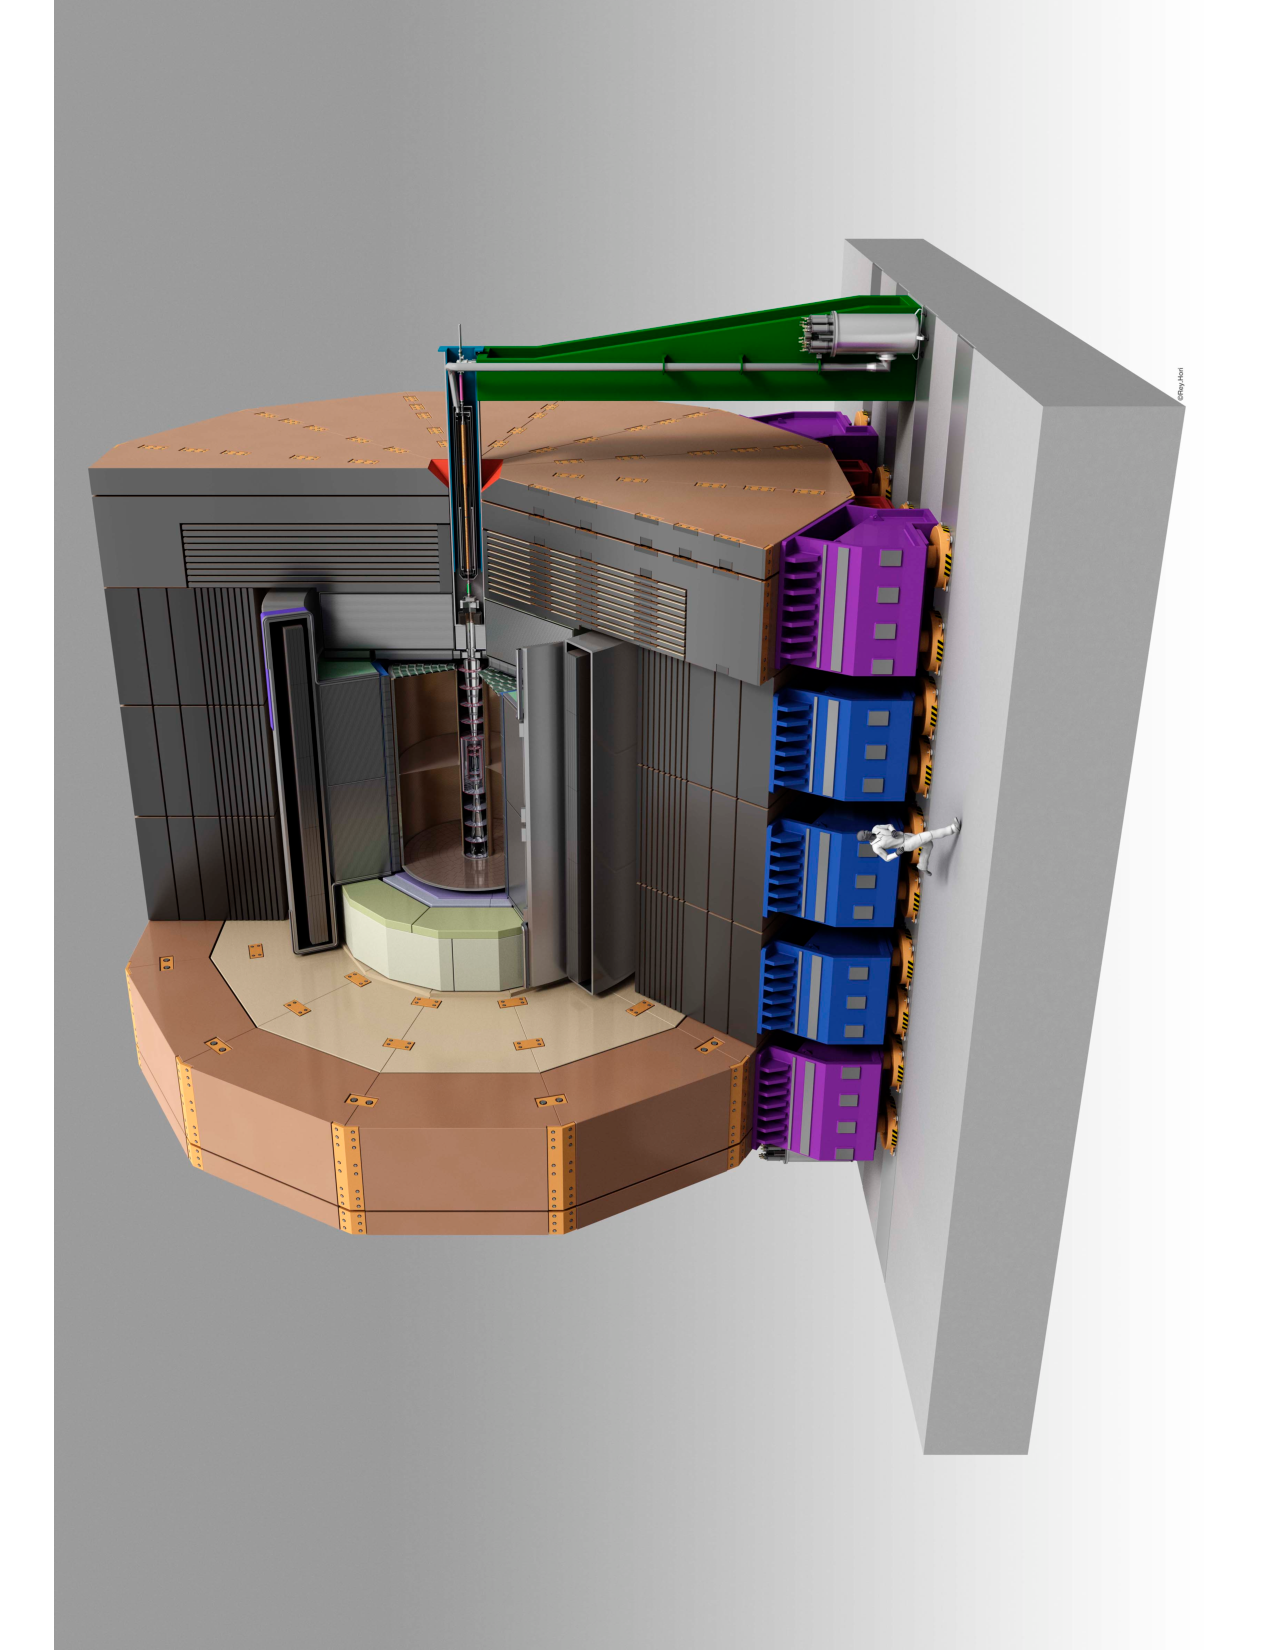
\includegraphics[width=0.48\hsize,clip]{figures/ILD.pdf} & 
 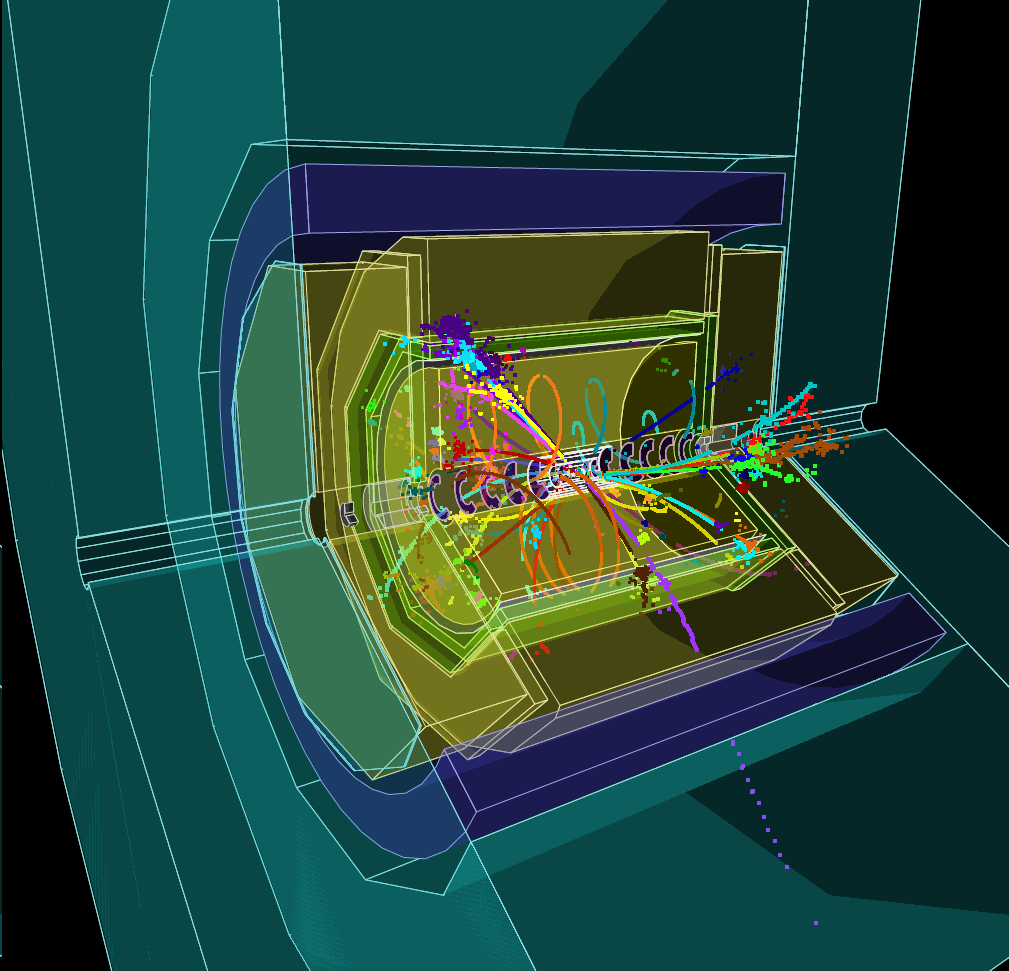
\includegraphics[width=0.35\hsize]{figures/tt_500GeV_3D.png}
 \\
 \end{tabular}
\caption{Left: Three-dimensional image of the ILD detector. Right: Event display of a simulated $t \bar t$ event in ILD.
\label{fig:ILD}}
 \end{center}
 \end{figure}


\subsection{Vertexing system}
The system closest to the interaction region is a pixel detector designed to reconstruct decay vertices of short lived particles with great precision. ILD has chosen a system consisting of three double layers of pixel detectors. The innermost layers is only half as long as the other ones, to reduce the number of background hits this layer is exposed to. Each layer will provide a spatial resolution around $4\mu m$ at a pitch of about $22 \mu m$, and a timing resolution per layer of around $2-4 \mu s$. Ongoing R\&D is directed towards allowing single bunch tagging per layer. 

Over the last 10 years the MAPS technology has matured to a point where all the requirements needed for an ILC detector can be met. The technology has seen a first large scale use in the STAR vertex detector~\cite{ild:bib:VTXcps3}, and, more recently, in the upgrade of the ALICE vertex detector. To minimize the material in the system the sensors are routinely thinned to 50 $\mu$ m. Very light weight support structures have been developed, which allow the goal of a radiation length per layer of around $0.1 \%$ to be in reach. 
Other technologies which are under investigation for the ILC detector are the DEPFET technology, which is currently being deployed in the BELLE II vertex detector~\cite{Luetticke:2017zpx}, the fine pitch CCD technology, and even less far developed concepts like SOI or Chronopix systems~\cite{RDliaision}. 

In figure~\ref{fig-btag} the purity of the flavour tag as a function of the efficiency is shown. In addition the system allows the determination of the vertex charge of detached vertices, and contribute strongly to the low-momentum tracking capabilities of the overall system, down to a few 10 MeV. 
\begin{figure}
    \centering
    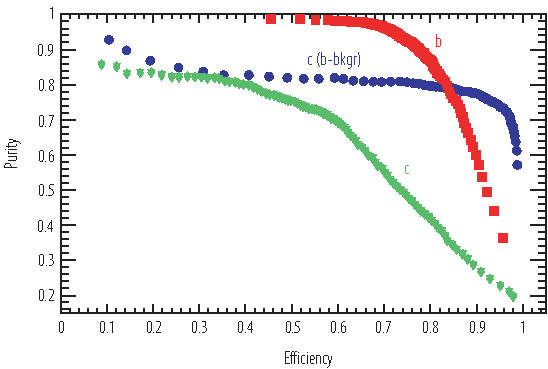
\includegraphics[width=0.45\hsize]{figures/FlavourTagPurities_Zpeak_DCR-eps-converted-to.pdf}
    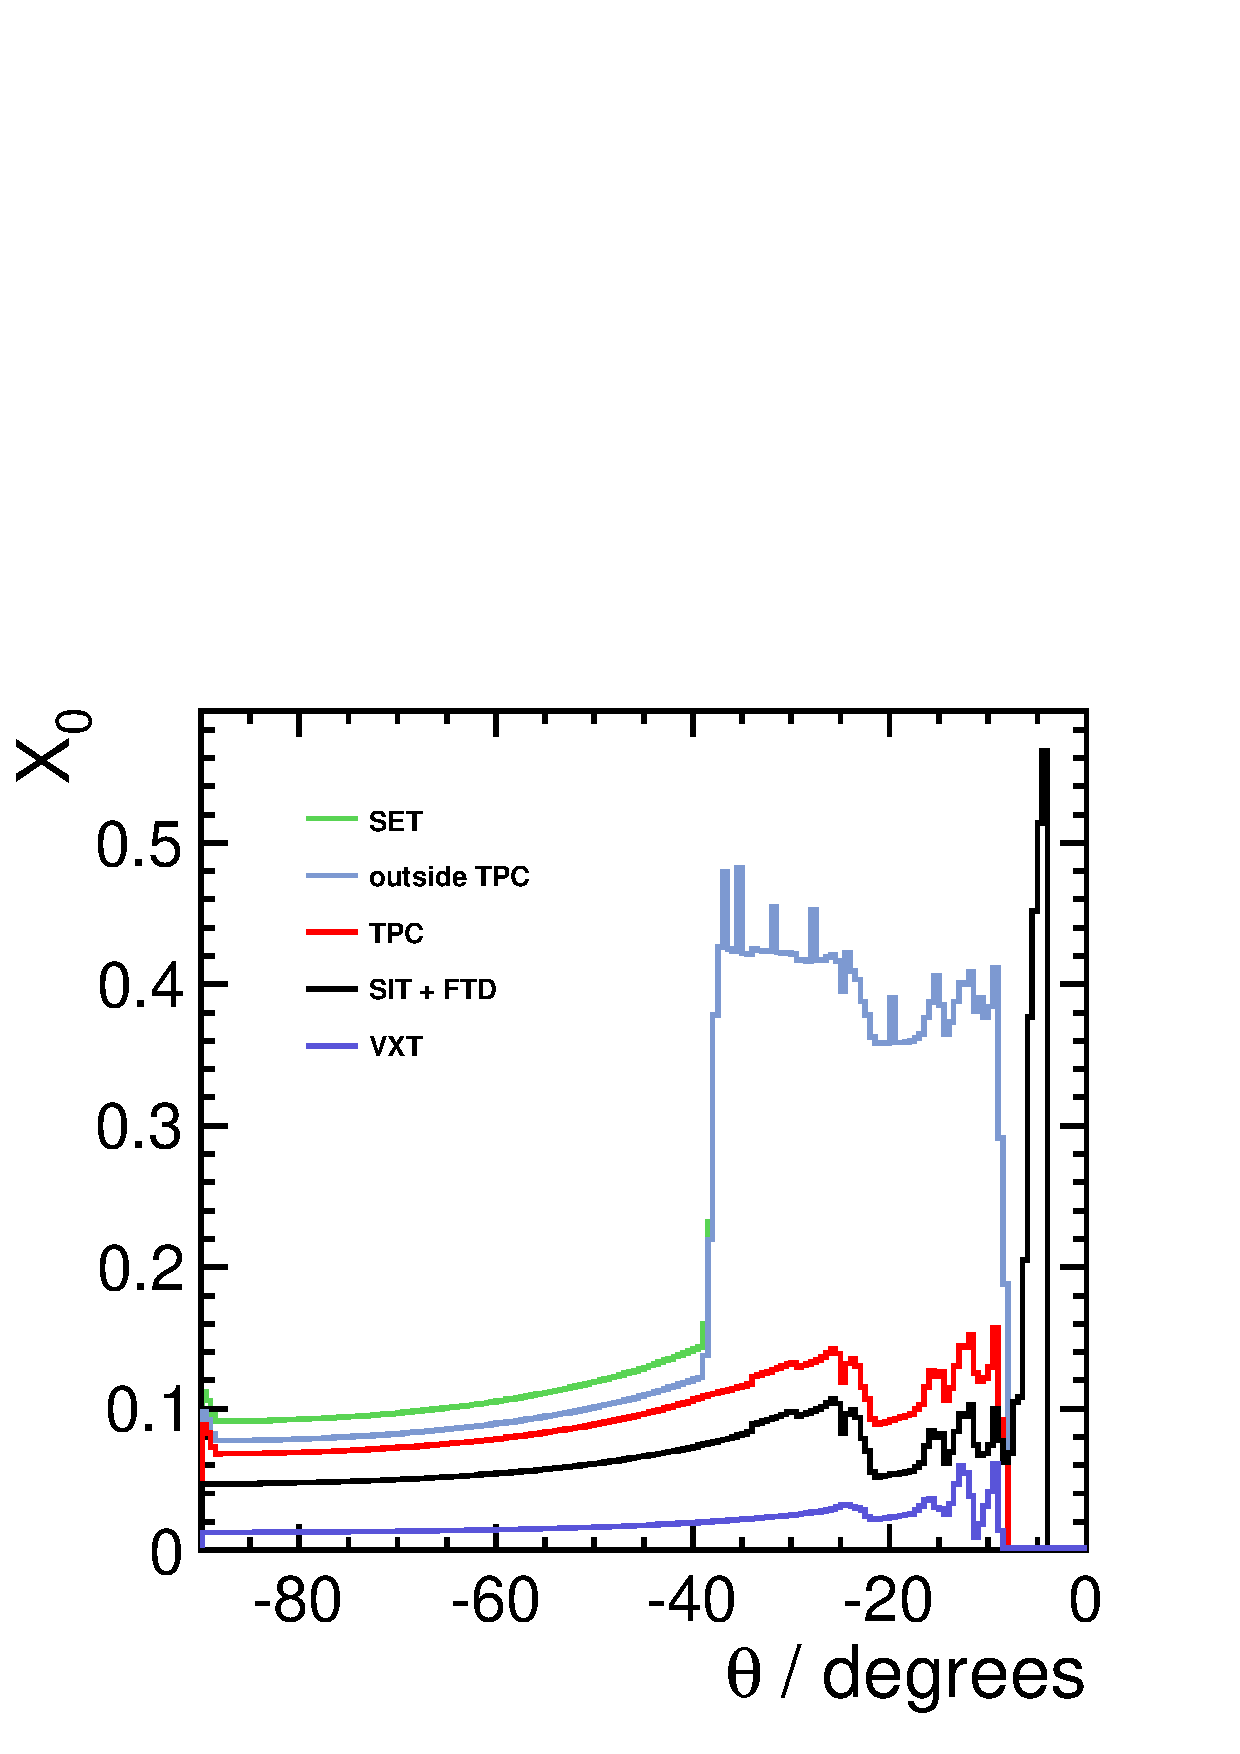
\includegraphics[width=0.35\hsize]{figures/material-budget-new.pdf}
    \caption{Left:Purity of the flavour tag as a function of the efficiency, for different flavours tagged. Right: Material budget in ILD up to the calorimeter.}
    \label{fig-btag}
\end{figure}  

\subsection{Tracking System}

Tracking of charged particles is a key requirement for the ILD detector. ILD has decided to approach the problem with a hybrid solution, which combines a high resolution time-projection chamber (TPC) with a few layers of strategically placed high resolution strip or pixel detectors before and after the TPC. 
The time projection chamber will fill a large volume of about 4.6~m length and spanning radii from 33 to 180~cm. In this volume the TPC provides in the barrel 220 three dimensional points, with a resolution of better than $100 \mu$m in $r \phi$, and about 1~mm in z. This large number of points allows a reconstruction of the charged particle component of the event with large accuracy, including the reconstruction of secondaries, long lived particles, kinks etc.. For momenta above 100 MeV nearly 100\% tracking efficiency has been found in event simulated realistically with full backgrounds. At the same time the complete TPC system will introduce only about 10\% of a radiation length into the detector~\cite{Diener:2012mc}. 

On the inside and on the outside of the TPC a few layers of Silicon detector provide additional high resolution points, which, once combined with the TPC track, will result in a momentum resolution of $2 \times 10^{-5}$ for the complete system. Since the dead material in the system is very low, a significantly better resolution at low momenta can be achieved than it is possible with a Silicon only tracker. This is illustrated in figure~\ref{fig:momentumvsp}, where the ILD resolution is shown as a function of the momentum of the charged particle. 

\begin{figure}
    \centering
    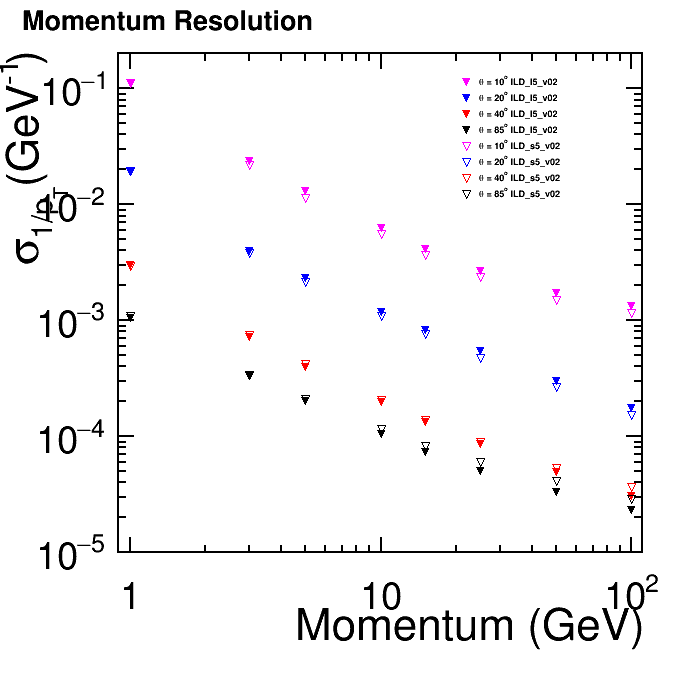
\includegraphics[width=0.38\hsize]{figures/PResolution_ILD_ls5_v02.png}
        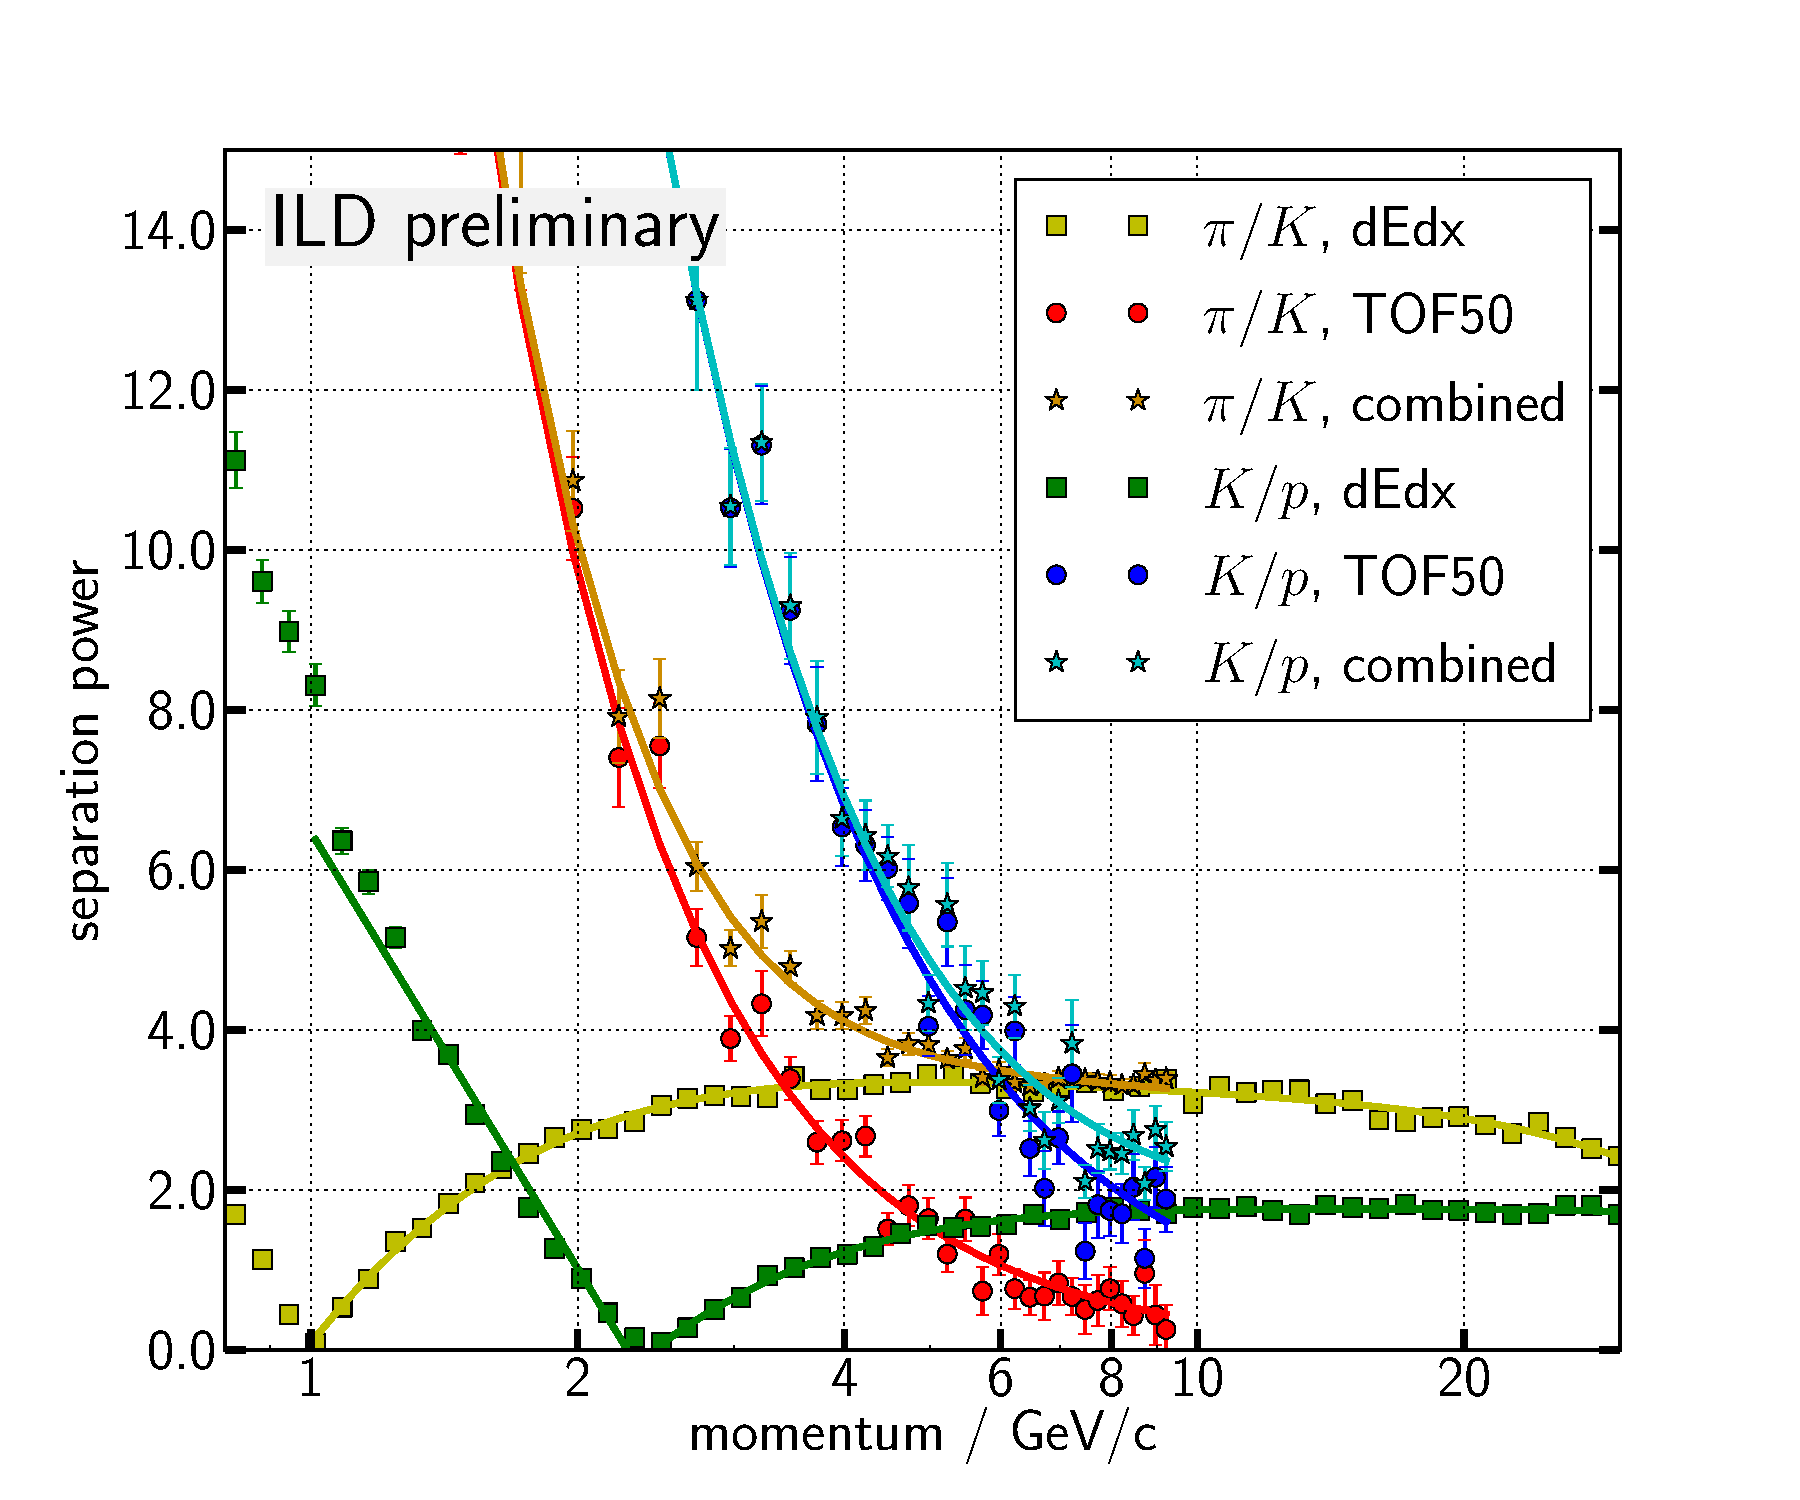
\includegraphics[width=0.55\hsize]{figures/Combined_dEdx_TOF50.pdf}
    \caption{ Left: Simulated momentum resolution as a function of the transverse momentum. The different curves correspond to different angular cuts, and to different detector models. right: Simulated separation power between pions and Kaons, from dEdx and from timing, assuming a 50ns timing resolution.}
    \label{fig:momentumvsp}
\end{figure}

The time projection chamber allows an identification of the particle type through the measurement of the specific energy loss, dE/dx, for tracks at intermediate momenta~\cite{Hauschild:2000eg}. The achievable resolution is shown in figure~\ref{fig:momentumvsp} (left). If the inner and/ or outer silicon layers can provide a timing of the particle at the level of 100 ps, the particle identification through dE/dx can be supplemented by time of flight measurements, which are particularly effective in the momentum regime which is problematic for dE/dx. This is shown by the second curve in figure~\ref{fig:momentumvsp} (right). 

The performance of the time projection chamber has been the subject of intense R\&D over the last 15 years. Several technologies for the readout of the TPC have been successfully developed, and have demonstrated the needed performance in test beam experiments. A large volume field cage has been built, to demonstrate the low mass technology needed to meet the 10\% goal discussed above. Most recently the performance of the specific energy loss, dE/dx, has been validated in test beam data. Based on these results, the TPC technology is mature for use in the ILD detector, and can deliver the needed performance (see e.g. \cite{Attie:2016yeu, Bouchez:2007pe}, . 


\subsection{Calorimeter System}
At the core of each particle flow detector is a very powerful calorimeter system. Particle flow stresses the capabilities of separating the individual particles in a jet, both charged and neutral. This puts the imaging capabilities at a premium, and pushes the calorimeter development in the direction of very high granularity of the system. A particularly challenging part is the precise reconstruction of the neutral hadronic component in the shower. A highly granular sampling calorimeter for the hadronic part is the answer by ILD on this challenge. The technological and conceptual development of the particle flow calorimeter have been largely done by the CALICE collaboration. 

ILD has chosen a sampling calorimeter readout with silicon diodes as one option for the electromagnetic calorimeter. Diodes with pads of about $5 \times 5$ mm$^2$ are used, to sample a shower 28 times in the electromagnetic section. In 2018 a test beam experiment could demonstrate the large scale feasibility of this technology, by showing not only that the anticipated resolution can be reached, but also by demonstrating that a system the size of the ILD detector can be build and operated. 

As an alternative to the Silicon based system, sensitive layers made from thin scintillator strips are also investigated. 

For the hadronic part of the ILD detector, two technologies are studies: a Silicon photo diode (SiPM) on scintillator tile technology\cite{Simon:2010mi}, and a version based on resistive plate chamber based readout~\cite{Laktineh:2010zsa}. The SiPM- on - tile option works with moderate granularity, of about $3 \times 3$ cm$^2$ tiles, and provides an analogue readout of the signal in each tile (AHCAL). The RPC technology has a better granularity, of $1 \times 1$ cm$^2$, but provides only limited amplitude information, equivalent to 2 bits (SDHCAL). For both technologies significant prototypes have been built and operated. Both follow the engineering design anticipated for the final detector, and demonstrate thus not only the performance, but also the scalability of the technology to a large detector. Particular challenges were the handling of the large number of channels, which requires the integration of a large part of the readout technology into the sensitive plane, and the operation of large area systems, including the handling of connected noise and timing issues. 

It has been a major success in the past years that the technologies needed for a true particle flow calorimeter have been successfully demonstrated, in a design which is suitable for the ILD detector. With this demonstration a major hurdle towards the realization of ILD has been surpassed ~\cite{Sefkow:2015hna}. The simulated particle flow performance is shown in figure~\ref{fig:pflow}.
\begin{figure}[th]
    \centering
    \begin{tabular}{lr}
    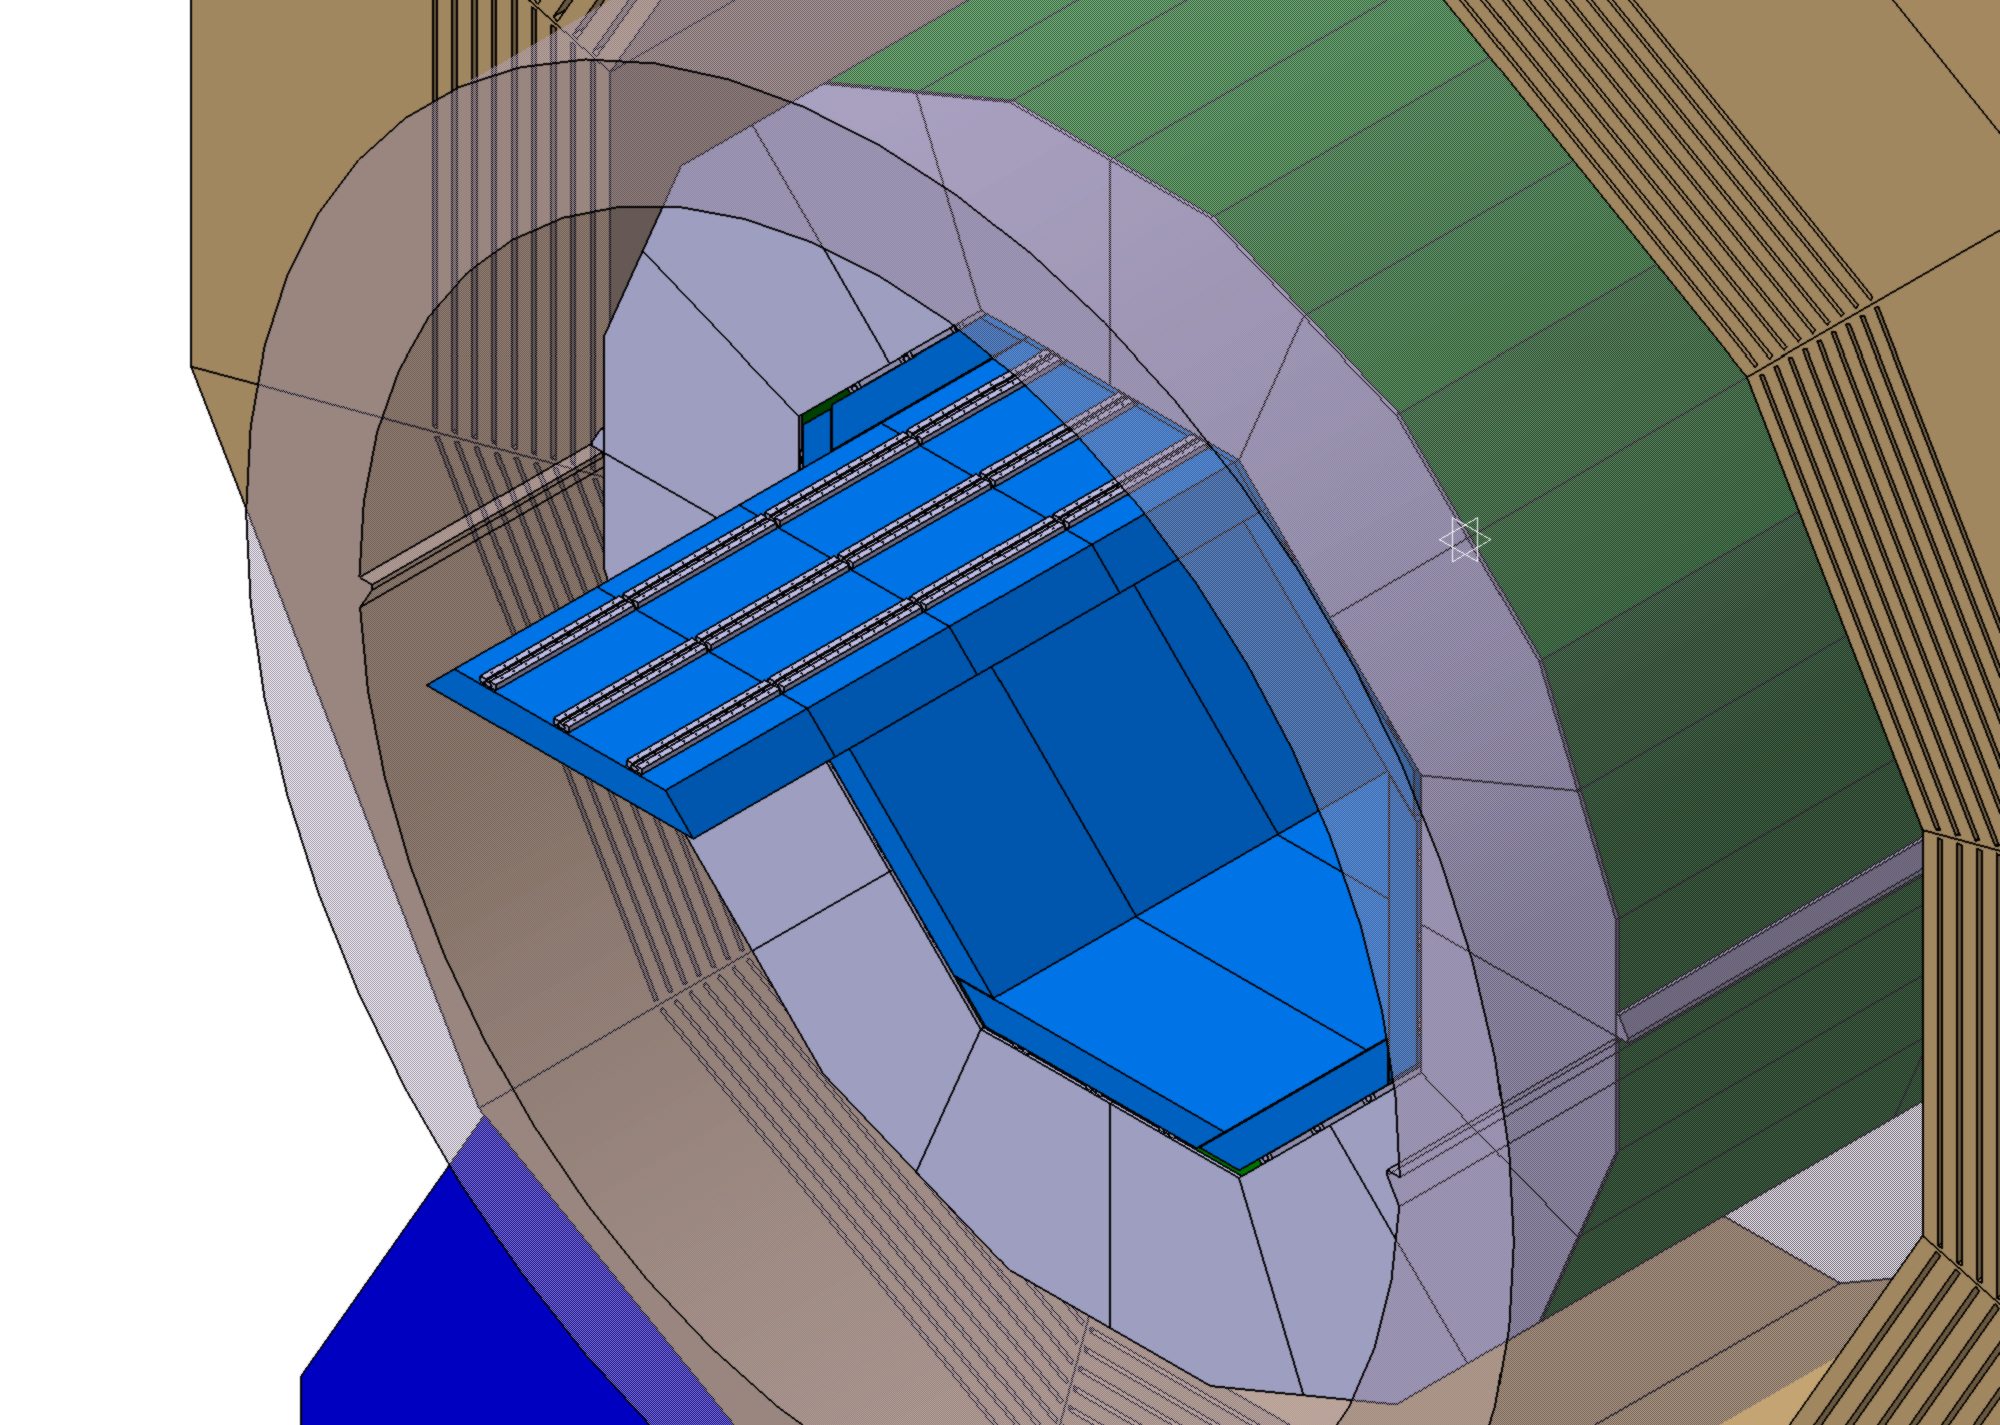
\includegraphics[width=0.45\hsize]{figures/ECal_insertion.jpg}&
    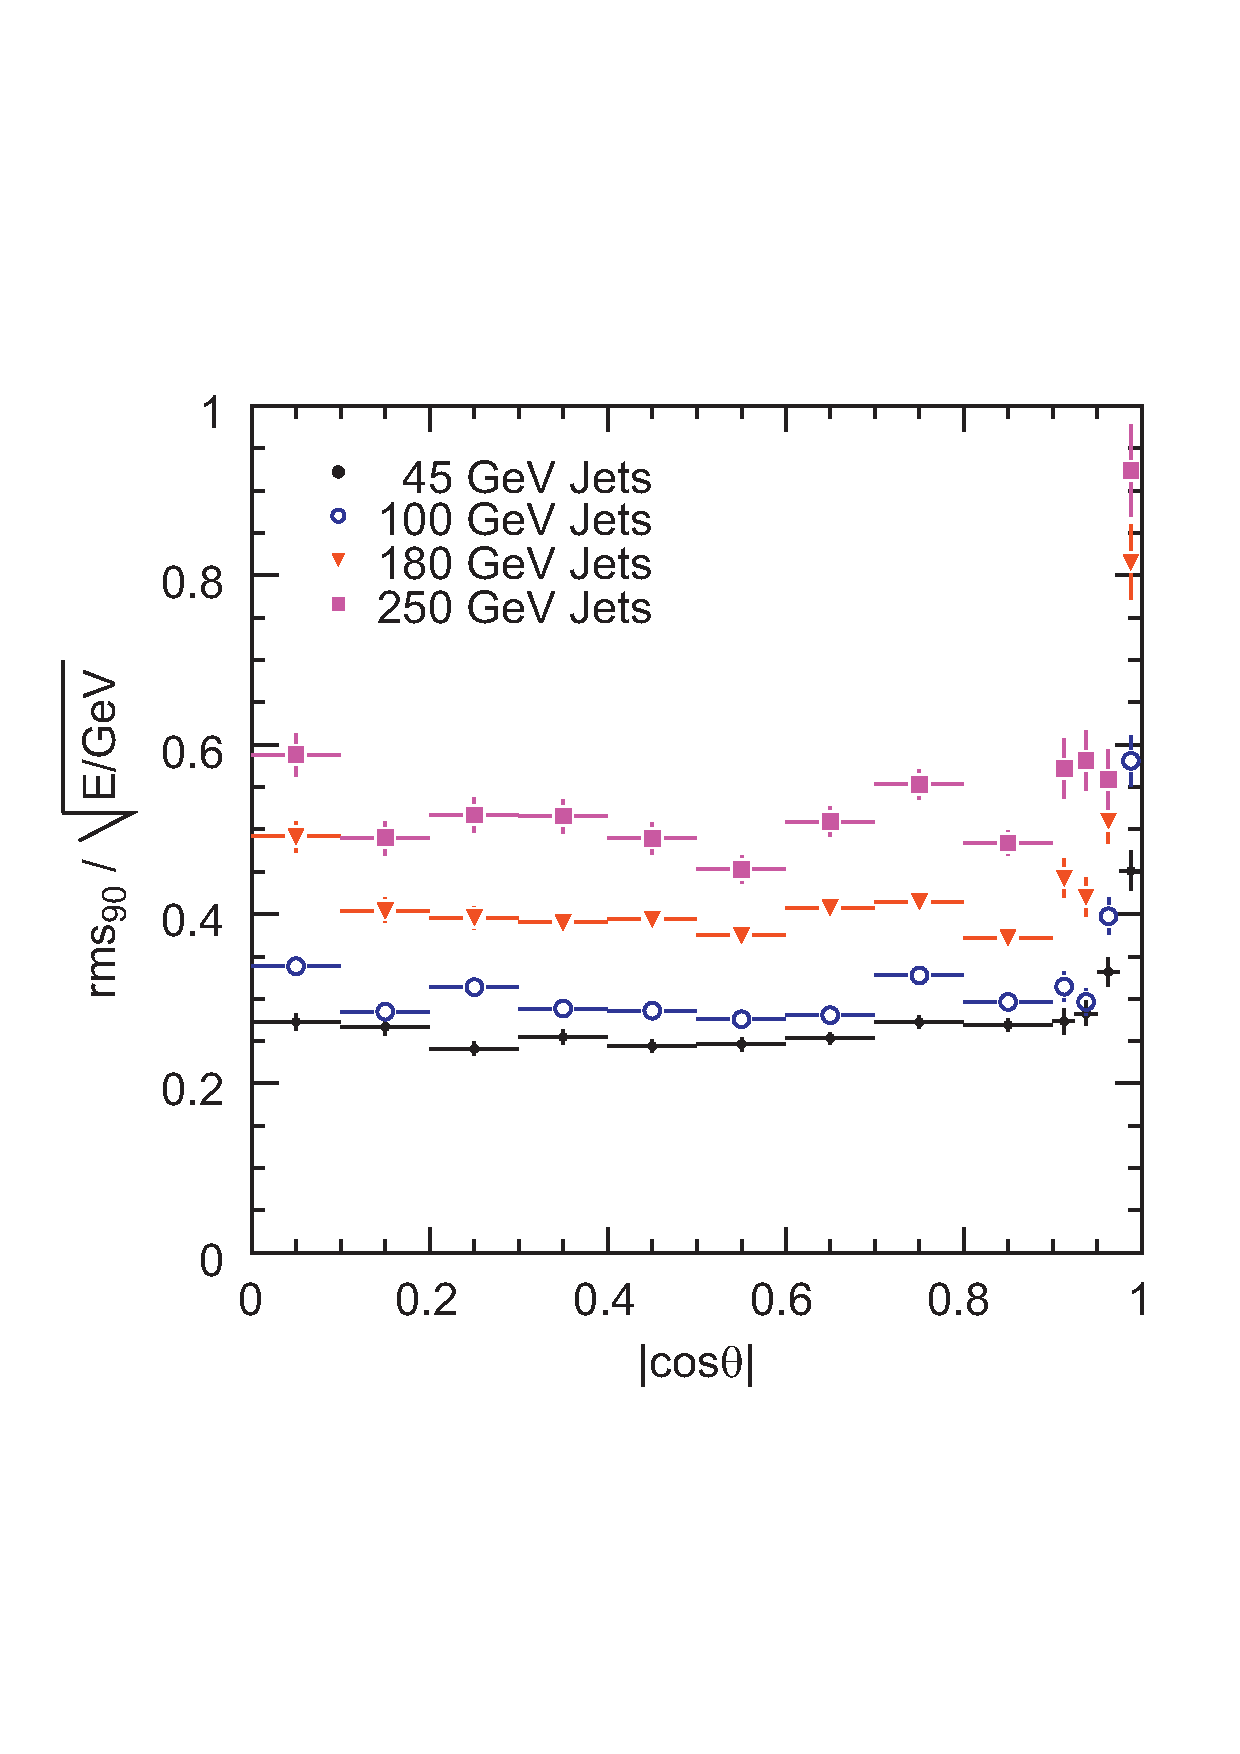
\includegraphics[width=0.4\hsize]{figures/pflow.pdf}\\
    \end{tabular}
    \caption{Left: Three-dimensional rendering of the barrel calorimeter system, with one ECAL module partially extracted. Right: Particle flow performance, measured as the energy resolution in two-jet light flavour events, for different jet energies. The resolution is defined as the rms of the distribution truncated so tha t$90$ of the total jet energy are contained inside the distribution.}
    \label{fig:pflow}
\end{figure}

\subsection{The Forward System}
Three rather specific calorimeter systems are foreseen for the very forward region of the ILD detector~\cite{Abramowicz:2010bg}. The LHCAL extends the reach of the endcap hadronic calorimeter system downwards towards smaller angels relative to the beam, and closes the gap between the octogonal geometry of the HCAL endcap and the round geometry of the luminosity calorimeter, Lumical. Lumical, a high precision fine sampling Silicon tungsten calorimeter is primarily designed to measure electrons from Bhabha scattering, to determine precisely the luminosity. Below the Lumkical acceptance, where background from beamstrahlung rises sharply, beamcal places further downstream from the interaction point, provides further coverage. As the systems move close to the beampipe, the requirements on radiation hardness and on speed become more and more challenging. Indeed this very forward region in ILD is the only region where radiation hardness of the systems is a key requirement. In placing the different detector components, particular care has been taken to allow the bulk of the beamstrahlungs photons and pairs to leave the detector through the outgoing beampipe hole. In particular the beamcal has been positioned in such a way that backscattering of particles from the beamcal face into the active part of the detector is minimised.

\subsection{Detector Integration and Costing}
One of the major goals of the ILD collaboration was from the beginning to push the detector concept from a collection of technological ideas to a real detector that can actually be built, commissioned, and operated within given engineering and site dependent constraints. The effort, driven by dedicated working groups, resulted in an engineering model of ILD that describes the mechanical setup of the detector structures themselves as well as the detector services as cabling, cooling, gas systems, and cryogenics. The technical description of ILD is based on Interface Control Documents and is documented on the ILC-EDMS system with a web-based front-end~\cite{EDMS}. A detailed CAD model of ILD exists and can be accessed a the same location.

The main mechanical structure of the ILD detector is the iron yoke that consists of three barrel rings and two endcaps. The yoke provides the required shielding for radiation and magnetic fields to allow access to the outside of the detector during data taking. The central yoke ring carries the cryostat for the detector soleniod and the barrel detectors, calorimeters and tracking system. The yoke endcaps carry the endcap detectors and can be opened to allow for access to the inner detector. The mechanical concept of ILD has been designed and tested in simulations for seismic conditions that can be expected at the foreseen ILC site in northern Japan.

A common concept for the detector services as cables, cooling, gases and cryogenics has been developed. The requirements are in many cases based on engineering prototypes of the ILD sub-systems. 

The main detector solenoid is based on the CMS experience and can deliver magnetic fields up to 4T. A correction system for the compensation of the crossing angle of the ILC beam, the Detector Integrated Dipole, has been designed and can be integrated into the main magnet cryostat.

The cost of the ILD detector has been estimated at the time of the ILD technical design report. The total detector cost has been found to be about $390 $ Mio ILCU in 2013 costs. One ILCU has been defined to be approximately equal to one dollar or 0.97 EUR in 2013. The cost of the detector is strongly dominated by the cost of the calorimeter system, and the iron return yoke, which together acount for about $60\%$ of the total cost. Currently an effort is ongoing to re-evaluate the cost. In addition to the detector described in this document, a smaller version of ILD is also considered, which will reduce the cost between $10$ and $20\%$. 

\section{Science with ILD}
ILD has been designed to operate at electron positron collisions between 250 GeV and 1 TeV. The science goals of the ILC have been described in detail in \cite{ILCESU1}, and will not be repeated here. It should be pointed out that the analyses which have been performed within the ILD group are based on fully simulated events, reconstructed with a realistic detector model and reconstruction software, and in many cases includes estimates of key systematic effects. This is particularly important when estimating the reach the ILC and ILD will have for specific measurements. Determining for example the branching ratios of the Higgs at the percent level depends critically on the detector performance, and thus, on the quality of the event simulation and reconstruction. 

In many cases the performance used in the physics analyses has been tested against prototype experiments. The key performance numbers for the vertexing, tracking and calorimeter system are all based on results from test beam experiments. The particle flow performance, a key aspect of the ILD physics reach, could not be fully verified, but key aspects have been shown in experiments. This includes the single particle resolution for neutral and charged particles, the particle separation in jets, the linking power between tracking and calorimetry, and key aspects of detailed shower analyses important for particle flow. 

In recent years the ILD collaboration has initiated a systematic benchmarking effort, to study the performance of the ILD concept, and to determine in particular the correlations between science objectives and detector performance. The list of benchmark analyses which are under study is given in Table \ref{tab-benchmark}. 

\begin{table}[thb]
    \centering
    \begin{tabular}{p{4cm}|p{5cm}|p {5cm}}
\hline
    Reaction     & Main physics question & main issue addressed \\
\hline
Higgs mass in $H\rightarrow b {\bar b}$         &  precision Higgs mass determination &Flavour tag, jet energy resolution  \\
\hline
Branching ratio $H \rightarrow \mu^+\mu^-$ & rare decay, Higgs Yukawa coupling to muons & sensitive to momentum resolution \\
\hline
Limit on $H \rightarrow$ invisible & Search for hidden sector & Jet energy resolution, Z or recoil mass resolution, hermeticity\\
\hline
Coupling between Z and left-handed $\tau$ & Contact interactions, BSM physics, & highly boosted topologies, $\tau$ reconstruction \\
\hline
$WW$ production, $W$ mass & anomalous couplings, W mass&  Jet energy resolution, impact of beamstrahlung on physics \\
\hline
Cross section of $e^+e^- \rightarrow \nu \nu qqqq$ & Test validity of SM at high energies &  W/Z separation, jet energy resolution, hermeticity\\
\hline
Left-Right asymmetry in $e^+e^- \rightarrow \gamma Z$ & SM validity &  jet energy scale calibration, lepton/ photon tagging \\
\hline
hadronic branching ratios for $H\rightarrow b \bar b $ and $d \bar c$ & Higgs mechanism &  flavour tag, jet energy resolution\\
\hline
discovery range for low $\Delta M$ Higgsinos & Testing SUSY in an area inaccessible for the LHC& tracks with very low $p_t$, ISR photon identification, finding multiple vertices\\
\hline
discovery range for WIMP's in mono-photon channel & WIMP models & Photon detection at all angles, tagging power in the very forward calorimeters\\
\hline
discovery range for low-mass extra Higgs in $e^+e^- \rightarrow Zh$ & Low mass, Higgs like states & Isolated muon finding, ISR reconstruction.\\

\hline
\multicolumn{3}{l}{Running above the top threshold:}\\
\hline
$A_{FB}, A_{LR}$ from $t \bar t \rightarrow bb qqqq$ & Form factors, electroweak coupling & reconstruct multi-jet final states with jet and vertex charge\\



    \end{tabular}
    \caption{Table of benchmark reactions which are used by ILD to optimize the detector performance. The channel, the physics motivation, and the main detector performance parameters are given.}
    \label{tab-benchmark}
\end{table}
\section{Integration of ILD into the experimental environment}
ILD is designed to work in a push-pull system with another detector at a common ILC interaction region. In this scheme, ILD sits on a movable platform in the underground experimental hall. This platforms allows for a roll-in of ILD from the parking position into the beam and vice versa within a few hours. The detector can be fully opened and maintained in the parking position.

The current mechanical design of ILD assumes an initial assembly of the detector on the surface, similar as it has been done for CMS at LHC. A vertical shaft from the surface into the underground experimental cavern allows for a lowering of ILD in basically five segments, given by the five yoke rings.

ILD is designed to fully cope with the ILD beam conditions. The expected levels of beam induced backgrounds have been simulated and are seen to be on tolerable levels, e.g. for the vertex detectors. Careful shielding keep scattered backgrounds under control. Machine-wise, the design of the interaction region and the collimation system has been done to keep the external background sources at levels below the detector requirements.

ILD is self-shielding with respect to radiation and magnetic fields so that operation of surrounding equipment, e.g. for cryogenics, and maintenance outside of the detector is possible. Of paramount importance is the possibility to operate and maintain the second ILC push-pull detector in the underground cavern.

\section{The ILD Collaboration}
As described above the ILD collaboration started out as a fairly loosed organised group of scientists interested to explore the consequences the requirements imposed from the science at the ILC would make on a detector. With the delivery of the DBD in 2013 the group re-organised itself more along the lines of a traditional collaboration. The group gave itself a set of by-laws which goverened the function of hte group, and setup rules for the membership in ILD. Groups who wanted to be members of ILD needed to sign a memorandum of participation, a first step towards an eventual memorandum of understanding to contruct ILD, once the ILC has been approved. 

In total 72 groups from XX coutries signed the letter of participation in 2015. In 2018 membership was reconfirmed. A map showing the location of the ILD member institutes is shown in figure~\ref{ild-fig-membermap}.

\begin{figure}
    \centering
    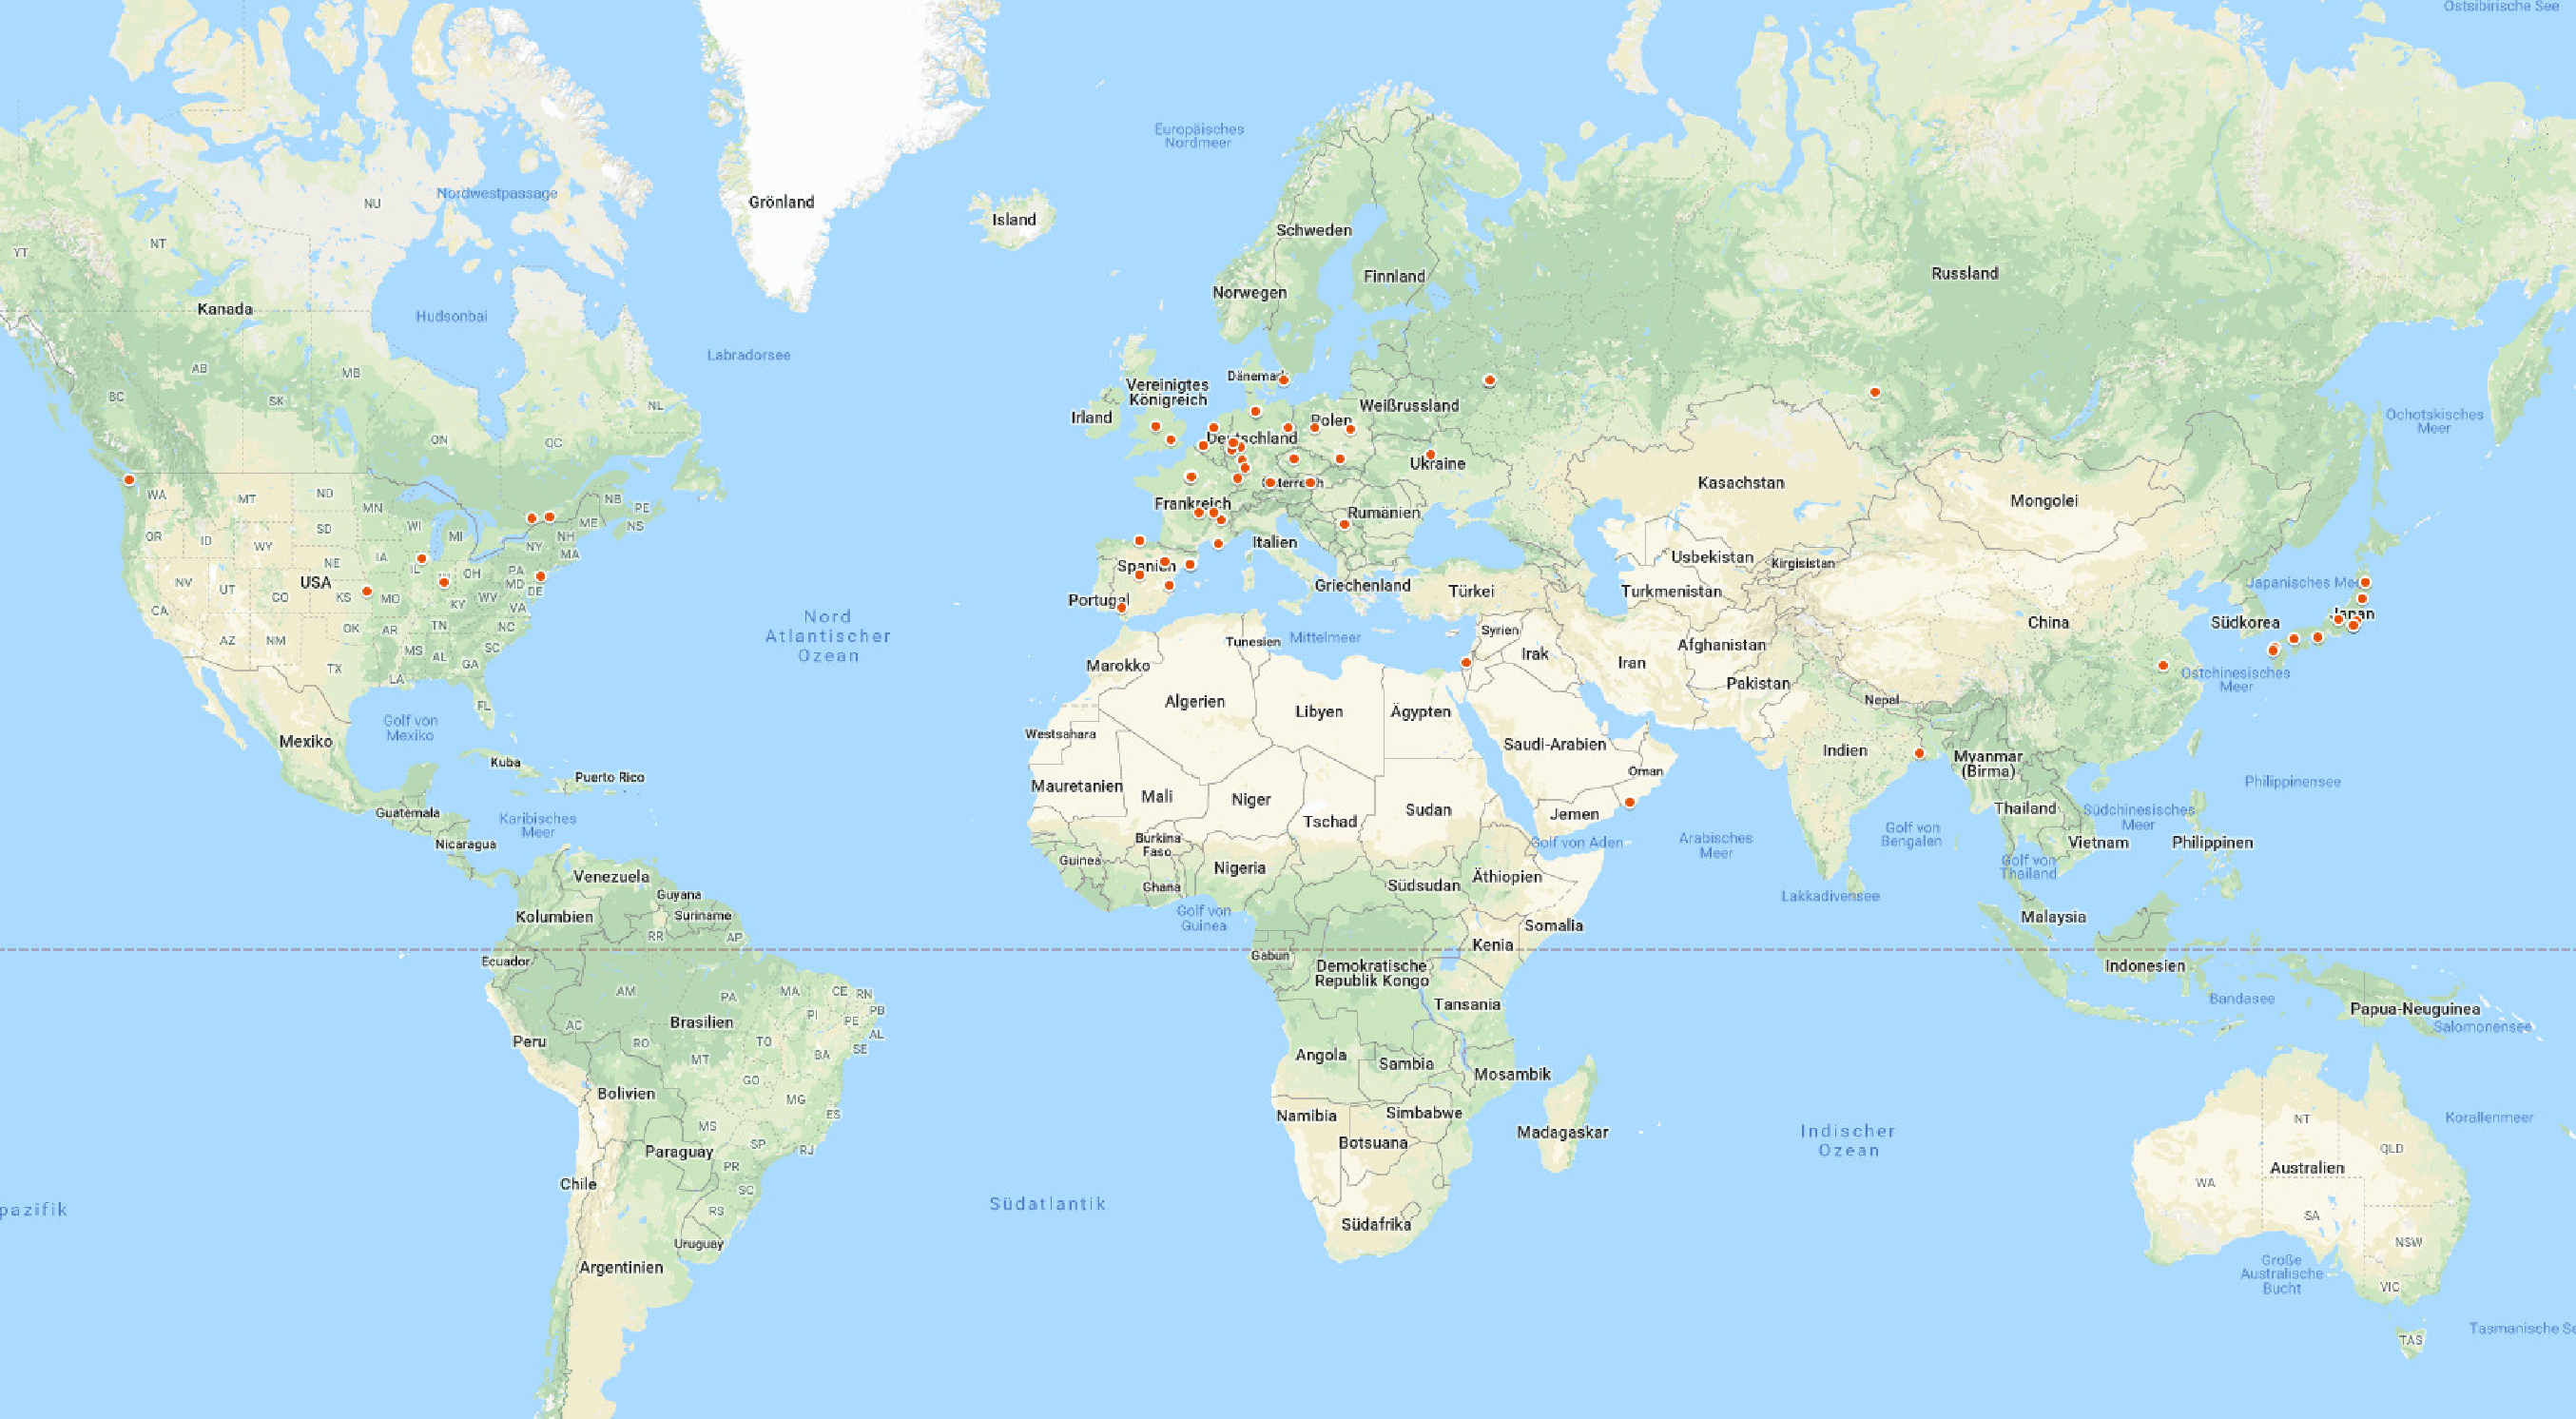
\includegraphics[width=0.6\hsize]{figures/ILD_members_map.pdf}
    \caption{Map with the location of the ILD member institutes indicated.}
    \label{ild-fig-membermap}
\end{figure}



\section{Conclusion and Outlook}
The ILD detector concept is a well developed integrated detector optimized for use at the electron positron collider ILC. It is based on advanced detector technology, and driven by the science requirements at the ILC. Most of its major components have been fully demonstrated through prototyping and test beam experiments. The physics performance of ILD has been simluated using detailed simulation systems. A community interested in building and operating ILD has formed over the last few years. It is already sizeable encompassing some 70 institutes from around the world. The community is ready to move forward once the ILC project receives a green light. 


\bibliography{ILD}
%\begin{thebibliography}{}
%\bibitem{EDMS} ILD Technical Documentation, %http://edmsdirect.desy.de/ildtdr

%\end{thebibliography}
\end{document}
%
% ****** End of file apssamp.tex ******